\documentclass[problem]{mcs}

\begin{pcomments}
  \pcomment{CP_Megumi_net}
  \pcomment{from: S09.miniquizapr9}
  \pcomment{check "plus two" remark re latency & diameter against current Notes}
\end{pcomments}

\pkeywords{
  networks
  Benes
  congestion
  routing
  latency
}

%%%%%%%%%%%%%%%%%%%%%%%%%%%%%%%%%%%%%%%%%%%%%%%%%%%%%%%%%%%%%%%%%%%%%
% Problem starts here
%%%%%%%%%%%%%%%%%%%%%%%%%%%%%%%%%%%%%%%%%%%%%%%%%%%%%%%%%%%%%%%%%%%%%

\begin{problem}
  Tired of being a TA, Megumi has decided to become famous by coming up
  with a new, better communication network design.  Her network has the
  following specifications: every input node will be sent to a Butterfly
  network, a Benes network and a 2D Grid network.  At the end, the outputs
  of all three networks will converge on the new output.

  In the Megumi-net a minimum latency routing does not have minimum
  congestion.  The \term{latency for min-congestion} (\term{LMC}) of a net
  is the best bound on latency achievable using routings that minimize
  congestion.  Likewise, the \term{congestion for min-latency}
  (\term{CML}) is the best bound on congestion achievable using routings
  that minimize latency.

\begin{center}
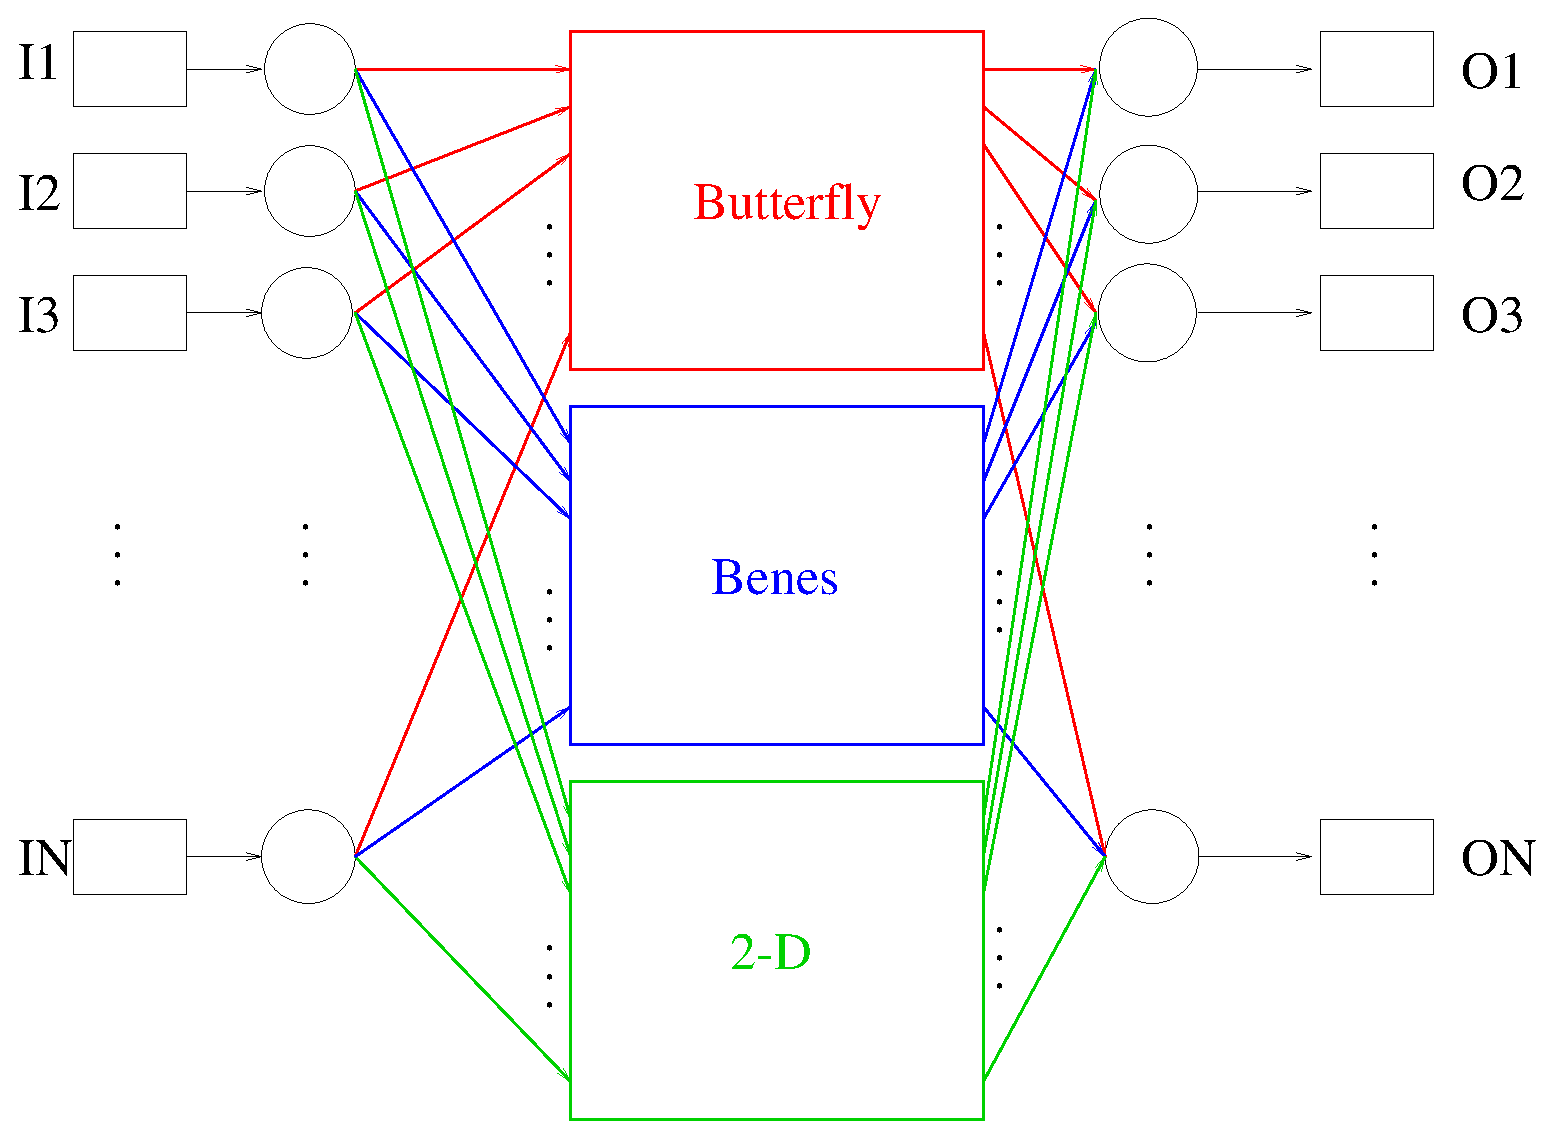
\includegraphics[width=4in]{mq4p2SP09}
\end{center}

Fill in the following chart for Megumi's new net and explain your answers.

\[
\begin{array}{|c|c|c|c|c|c|}
\hline
\textbf{network} &
\textbf{diameter} &
%\textbf{switch size} &
\textbf{\# switches} &
\textbf{congestion} &
\textbf{LMC} &
\textbf{CML} \\ \hline
%\text{complete binary tree} & 2 \log N + 2 & 3 \times 3 & 2N - 1 & N \\
%\text{2-D array} & 2 N & N^2 & 2 & 2 N & 2 \\
%\text{butterfly} & \log N + 2 & N (\log(N) + 1) & \sqrt{N}\iffalse \text{ or } \sqrt{N/2}\fi
% & \log N + 2 & \sqrt{N}\iffalse \text{ or } \sqrt{N/2}\fi\\
%\text{Bene\u{s}} & 2 \log N + 1 & 2 N \log N & 1 & 2 \log N + 1 & 1 \\ \hline
\text{Megumi's net} & 
%~~~~~~~~~~~~~~~~~~~~~~~~~~~~~~~~~~&
~~~~~~~~~~~~~~~~~~~~~~&
~~~~~~~~~~~~~~~~~~~~~~&
~~~~~~~~~~~~~~~~~~~~~~&
~~~~~~~~~~~~~~~~~~~~~~&
~~~~~~~~~~~~~~~~~~~~~~\\ \hline
\end{array}
\]

\begin{solution}

\[
\begin{array}{|c|c|c|c|c|}
\textbf{diameter} &
\textbf{\# switches} &
\textbf{congestion} &
\textbf{LMC}&
\textbf{CML}\\
\hline (\log N + 2) +2 & 3N (\log N + 1) + N^{2} & 1 & 2 \log N +
3 & \sqrt{N}\\
\hline
\end{array}
\]

The diameter and congestion of a composite network such as this is
the smallest of the diameters and congestions of the sub-networks - with
two added to the diameter for the input and output steps. 
The number of switches is simply the sum of the switches in all the
 networks plus $2N$ for the input and output switches, and the CML 
and LMC can be found by taking the congestion of the network with 
minimum diameter and the diameter of the network with minimum 
congestions ---again, plus two for the inputs and outputs.

%Check the "plus two" remark against current Notes

\end{solution}
\end{problem}

%%%%%%%%%%%%%%%%%%%%%%%%%%%%%%%%%%%%%%%%%%%%%%%%%%%%%%%%%%%%%%%%%%%%%
% Problem ends here
%%%%%%%%%%%%%%%%%%%%%%%%%%%%%%%%%%%%%%%%%%%%%%%%%%%%%%%%%%%%%%%%%%%%%

\endinput
